\documentclass[9pt]{pnas-new}
% Use the lineno option to display guide line numbers if required.
% Note that the use of elements such as single-column equations
% may affect the guide line number alignment. 

% \RequirePackage[english,slovene]{babel} % when writing in slovene
\RequirePackage[slovene,english]{babel} % when writing in english
\usepackage{subcaption}

\templatetype{pnasresearcharticle} % Choose template 
% {pnasresearcharticle} = Template for a two-column research article
% {pnasmathematics} = Template for a one-column mathematics article
% {pnasinvited} = Template for a PNAS invited submission

\selectlanguage{slovene}
% \etal{in sod.} % comment out when writing in english
\renewcommand{\Authands}{ in } % comment out when writing in english
\renewcommand{\Authand}{ in } % comment out when writing in english

\newcommand{\set}[1]{\ensuremath{\mathbf{#1}}}
\renewcommand{\vec}[1]{\ensuremath{\mathbf{#1}}}
\newcommand{\uvec}[1]{\ensuremath{\hat{\vec{#1}}}}
\newcommand{\const}[1]{{\ensuremath{\kappa_\mathrm{#1}}}} 

\newcommand{\num}[1]{#1}

\graphicspath{{./figures/}}

\title{Simulation-driven gym layout optimization}

% Use letters for affiliations, numbers to show equal authorship (if applicable) and to indicate the corresponding author
\author{Andrej Jočić}
\author{Matic Stare}
\author{Martin Starič}

\affil{Collective behaviour course research seminar report} 

% Please give the surname of the lead author for the running footer
\leadauthor{Jočić} 

\selectlanguage{english}

% Please add here a significance statement to explain the relevance of your work
\significancestatement{Significance statement}{This report describes our work on gym layout optimisation. We begin with a brief overview of the problem and related work, followed by a description of our model and simulation. We conclude with a discussion of our results and future work.}

\selectlanguage{english}

% Please include corresponding author, author contribution and author declaration information
%\authorcontributions{Please provide details of author contributions here.}
%\authordeclaration{Please declare any conflict of interest here.}
%\equalauthors{\textsuperscript{1}A.O.(Author One) and A.T. (Author Two) contributed equally to this work (remove if not applicable).}
%\correspondingauthor{\textsuperscript{2}To whom correspondence should be addressed. E-mail: author.two\@email.com}

% Keywords are not mandatory, but authors are strongly encouraged to provide them. If provided, please include two to five keywords, separated by the pipe symbol, e.g:
\keywords{gym layout | crowd simulation | gym-goer behaviour | gym traffic}
\begin{abstract}
This report describes our work on gym layout optimisation. We begin with a brief overview of the problem and related work, followed by a description of our model and simulation. We conclude with a discussion of our results and future work.
\end{abstract}

\dates{\textbf{\today}}
\program{BM-RI}
\vol{2023/24}
\no{CB:G1} % group ID
%\fraca{FRIteza/201516.130}

\begin{document}

% Optional adjustment to line up main text (after abstract) of first page with line numbers, when using both lineno and twocolumn options.
% You should only change this length when you've finalised the article contents.
\verticaladjustment{-2pt}

\maketitle
\thispagestyle{firststyle}
\ifthenelse{\boolean{shortarticle}}{\ifthenelse{\boolean{singlecolumn}}{\abscontentformatted}{\abscontent}}{}

% If your first paragraph (i.e. with the \dropcap) contains a list environment (quote, quotation, theorem, definition, enumerate, itemize...), the line after the list may have some extra indentation. If this is the case, add \parshape=0 to the end of the list environment.
\section*{Introduction}
% \dropcap{I}
In this report we describe our work on gym layout optimisation.
A common occurrence in gyms during peak hours is over-crowding of popular equipment and lots of wandering around searching for a free machine.
Through simulating gym-goer behavior, we aimed to identify the most effective arrangement of exercise equipment to improve the flow, accessibility, and overall customer satisfaction.
Our goal is to offer practical insights for gym owners, managers, and designers seeking to optimize their facility layout for the benefit of their clients and business success.

To simplify the problem
we will limit ourselves to simulating the behaviour of bodybuilders (performing resistance exercises for muscle hypertrophy).
In this case, a typical workout routine partitions the body into several sets of muscles, cycling through them on a per-workout basis.
%This rotation can be done on a weekly schedule, or the workouts can be weekday-independent for greater flexibility. Popular splits include:
To further simplify the problem, we will only simulate the
\textit{push-pull-legs} (PPL) partitioning, which is a popular choice for beginners and intermediate lifters.
We will model the gym as a rectangular grid of cells with pre-set equipment locations, distributed similarly as isles in a grocery store.
%  - Push muscles are those involved in pushing movements,
% 	such as the chest, frontal deltoids (shoulders), and triceps. Pull muscles are those involved in pulling movements, such as the back musculature, rear deltoids, and biceps. Legs are the lower body muscles, such as the quadriceps, hamstrings, and calves.
% \end{itemize}


\subsection*{Related work}
The only publication related to gym layout optimization we could find was ref. \cite{turcine2022gym}, which assumed all gym clients had fixed-order workout routines (including ones with weight loss as a goal) and optimised a circular gym layout to minimise backward movement. Unfortunately, this does not give a good foundation for our work, as the assumptions diverge too far from what we are trying to model.

Thus we started from a crowd modelling review \cite{yang2020crowd_modelling_review} for basic model design principles. We also found two useful articles about incremental urban layout optimisation \cite{feng2016crowd_drive_layout_design, mathew2019urban_walkability} for inspiration.

\section*{Methods}

We used Python's {\it Mesa} library for simulation, analysis, and visualization of agent-based models.

\subsection*{Gym layout model}

A gym is represented as a subclass of \texttt{mesa.Model} with two discrete rectangular grids: the agent layer (where gym-goers move around) and the equipment layer (where machines are statically placed for one simulation cycle). The agents can only move around in cells that are not occupied by a piece of equipment, but there can be multiple agents in a single cell. We do not feel that agent collision resolution is necessary for realistic modelling of gym traffic. 
One corner of the area serves as the locker area entrance, where agents enter and exit the gym.

For generating a concrete placement of machines, we have to assign certain cells to be equipment locations (where one machine is placed) while making sure we don't create unreachable areas. For a start, we will develop some layout templates mimicking the arrangement of isles in a grocery store, with sensible walkways in between. In this case, layout optimisation comes down to choosing the best assignment of machines to equipment locations.

\subsection*{Gym-goer behaviour model}

A gym-goer is represented as a subclass of \texttt{mesa.Agent} with a training checklist (multiset of muscles) and its current state.  The agent's goal is to exhaust the checklist as quickly as possible and exit the gym.

When an agent is created, it is assigned a workout routine (eg. push) and a workout plan (eg. chest, chest, triceps, frontal deltoids). Routines will be sampled with probabilities based on our observations of people in our local gyms. The workout plans are constructed ad hoc, in keeping with general workout programming practice.

Upon entering the gym, an agent starts in state {\it searching}, where it looks for a free piece of equipment it can use to check  any item off its checklist. In the current implementation, the agent moves around randomly until an appropriate machine appears in its field of view (as defined by a radius $r$ where $r=1$ means the 8 neighboring cells).
In the future, we will implement more realistic searching movement, such as walking along a pre-defined exploration path around the gym (which for the right kind of layout template could be an eulerian cycle through corridors in the equipment layer), or actual pathfinding to the nearest free machine.

When a free machine is found, the agent enters state {\it exercising} and occupies the machine for a certain amount of time.
After the time has elapsed, the agent re-enters state {\it searching} or exits the gym if the checklist is empty.


\subsection*{Layout optimisation}

We have not yet decided on a specific optimisation algorithm, but here we outline some of the possibilities we are considering.

We will begin the opitimisation with a random layout (or set of layouts) and apply some local optimisation. Given the right kind of layout template, we could try genetic algorithms.
Alternatively, we will consider the Metropolis-Hastings algorithm which was successfully applied to urban layout optimisation \cite
{feng2016crowd_drive_layout_design,mathew2019urban_walkability}.

\subsubsection*{Objective function}

The quality of a layout will be measured as a weighted sum of the following factors (determined in a simulation cycle): 
\begin{itemize}
	\item proportion of time spent exercising (vs. searching or waiting around),
	\item local gym crowdedness (eg. maximum number of agents in a single cell), and
	\item an agent's ability to finish its workout in the amount of time it has available (eg. 1 hour).
\end{itemize}
We might also consider the cost of equipment (and its installation), though this is difficult to estimate in general and might make more sense as an input to our optimiser, given by a gym designer.


\section*{Results}

We started by trying to optimize gym layout with 2 machine islands. 


\begin{figure}[H]
	\begin{subfigure}{0.495\linewidth}
        \centering
        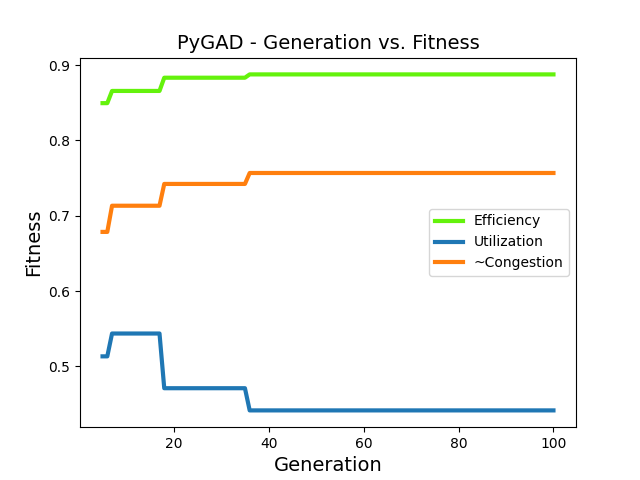
\includegraphics[width=\textwidth]{fitness_1.png}
        \caption{Graph representing layout evolution.}\label{fig:fitness_1}
    \end{subfigure}
    \begin{subfigure}{0.495\linewidth}
        \centering
        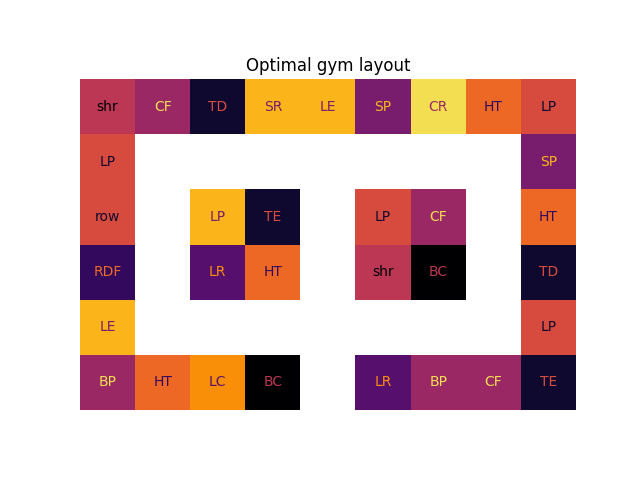
\includegraphics[width=\textwidth]{layout_1.png}
        \caption{Result layout of 2 machine islands.}\label{fig:layout_1}
    \end{subfigure}
    \caption{First test.}\label{fig:firstTest}
\end{figure}



\begin{figure}[H]
	\begin{subfigure}{0.495\linewidth}
        \centering
        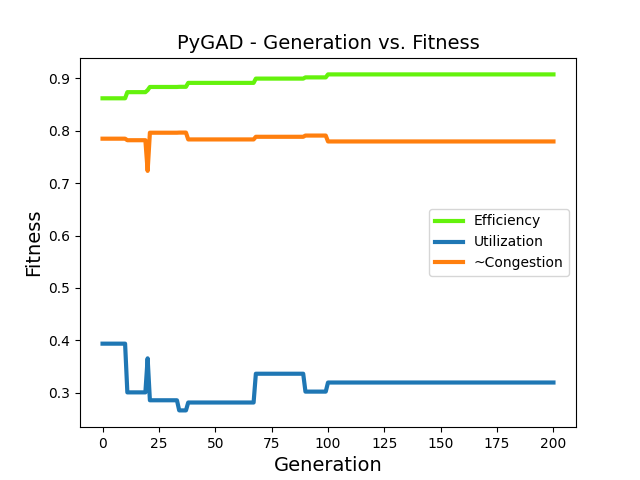
\includegraphics[width=\textwidth]{2x2fitness.png}
        \caption{Graph representing layout evolution.}\label{fig:2x2fitness}
    \end{subfigure}
    \begin{subfigure}{0.495\linewidth}
        \centering
        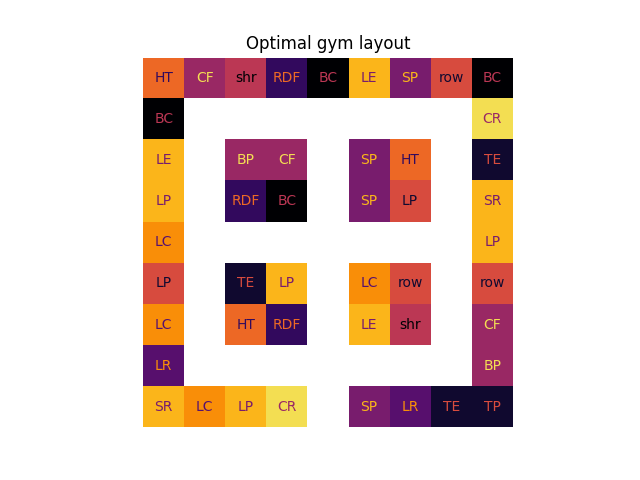
\includegraphics[width=\textwidth]{2x2_layout.png}
        \caption{Result layout of 2 machine islands.}\label{fig:2x2_layout}
    \end{subfigure}
    \caption{Second test.}\label{fig:secondTest}
\end{figure}



\begin{figure}[H]
	\centering
	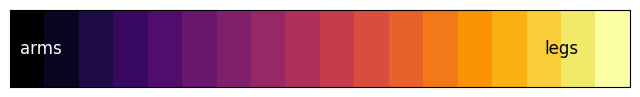
\includegraphics[width=\textwidth]{workoutTypeColormap.png}
	\caption{Colormap representing different muscles.}\label{fig:colormap}
\end{figure}


\section*{Discussion}

\subsection*{Future work} 

We could make our gym layout model more realistic with the addition of shared resources (eg. free weights next to a set of benches), compound machines (eg. a cable harness with multiple weight stacks) and multi-purpose equipment (eg. a squat rack with a pull-up bar), but none of this is a priority for now.
It might be a lot more interesting to let our optimizer come up with a layout from scratch (without hand-crafted templates), but it's likely this will make the optimizer take too long to converge to anything sensible.

We will also consider implementing more fine-grained agent behaviour, such as:
\begin{itemize}
	\item {\bf Parallel use of gym equipment:} A resistance exercise is usually performed as a sequence of (typically 3) {\it sets} where a movement is repeated some number of times, with short breaks in between. These breaks facilitate parallel use of gym equipment by two people, where one works out while the other rests. Note that this might involve time-consuming weight adjustment in between sets in case of differing strength levels, depending on the type of machine. Thus we will have to model a preference for free machines, even if it means greater travel distance for the agent.
	\item {\bf Non-uniform arrival of agents:} In the current implementation, a simulation starts with all agents entering the gym at the same time. We will implement a more realistic arrival process, where agents arrive at a time-dependent rate which peaks in the early evening.
	\item {\bf Smarter exercise selection:} An agent could exhibit preferences based on its immediate workout history. For example, it could try to avoid performing 2 chest exercises back-to-back in a push workout, since the chest fatigue will make the second exercise less effective.
	\item {\bf Larger timescale of simulation cycles:} If we simulated several days of gym traffic, we could have agents persist across workouts and thus actually cycle through their workout routines (such as push, pull, legs or some alternative partitioning) instead of just assigning each agent a random workout upon creation.
\end{itemize}

\acknow{Everyone worked on the report and gym-goer behaviour model. Andrej Jočić did stuff. Martin Starič implemented the pathfinding algorithm. Matic Stare made the project presentation.}

\showacknow % Display the acknowledgments section

% \pnasbreak splits and balances the columns before the references.
% If you see unexpected formatting errors, try commenting out this line
% as it can run into problems with floats and footnotes on the final page.
%\pnasbreak

\begin{multicols}{2}
\section*{\bibname}
% Bibliography
\bibliography{./bib/bibliography}
\end{multicols}

\end{document}